\thispagestyle{thachthuctoanhocnone}
\pagestyle{thachthuctoanhoc}
\everymath{\color{thachthuctoanhoc}}
\graphicspath{{../thachthuctoanhoc/pic/}}
\begingroup
\AddToShipoutPicture*{\put(0,616){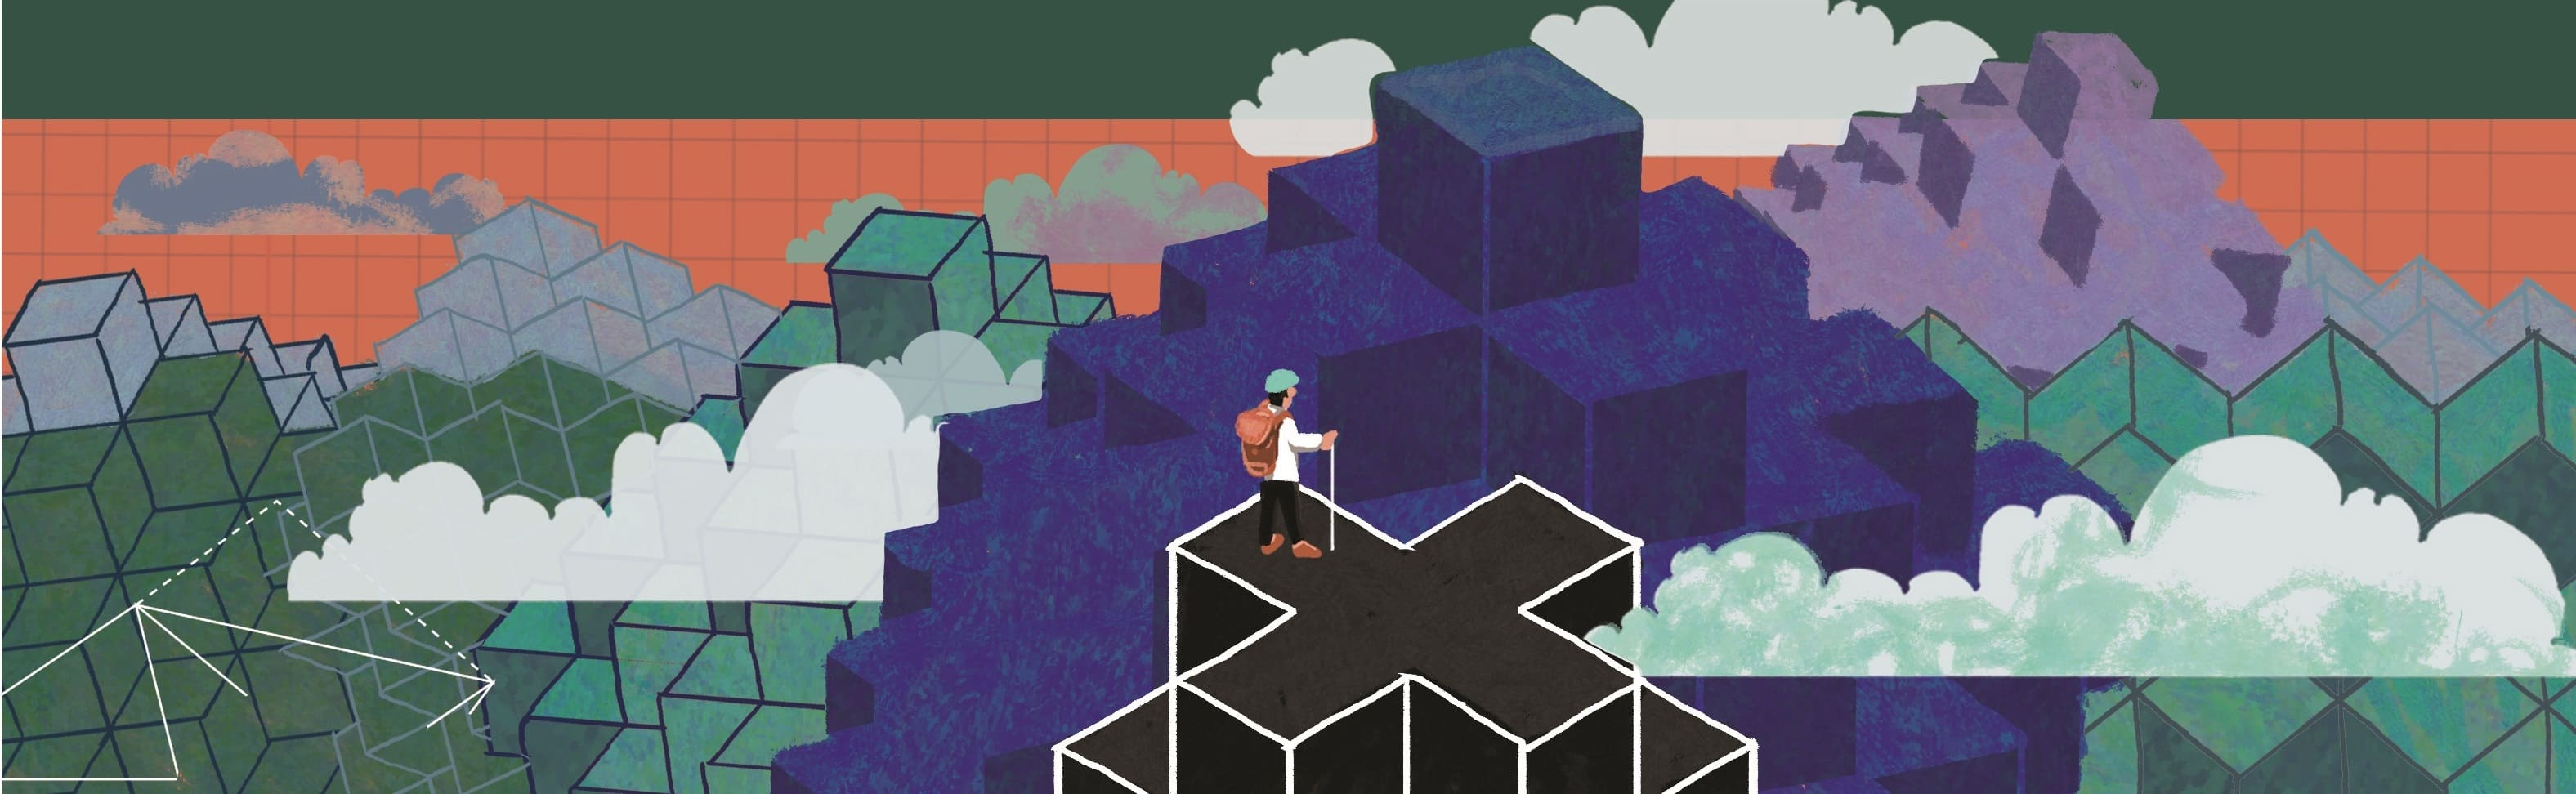
\includegraphics[width=19.3cm]{../thachthuctoanhoc/bannerthachthuc}}}
\centering
\vspace*{4cm}
\endgroup
\vspace*{-8pt}
\begin{tBox}
	\begin{itemize}[leftmargin = 13pt, itemsep = 1.0pt] 
		\item Mỗi bài toán đề xuất (kèm theo lời giải) cần được nêu rõ là bài sáng tác hay bài sưu tầm.
		%		\item Mỗi bài toán đề xuất (kèm theo lời giải) cần được nêu rõ là bài sáng tác hay bài sưu tầm (nếu là bài sưu tầm, cần ghi rõ nguồn).
		\item Bài giải cho mỗi bài toán cần được trình bày trong một file riêng hoặc
		một tờ giấy riêng.
		\item  Người đề xuất bài toán hoặc gửi bài giải cho các bài toán trong mục ``Thách thức kỳ này" cần ghi rõ họ, đệm, tên và nơi làm việc/học tập, số điện thoại liên hệ. Nếu là học sinh (hoặc sinh viên) cần ghi rõ là học sinh lớp mấy (hoặc sinh viên năm thứ mấy).
		\item Các bài toán trong mục Thách thức kỳ này hướng tới các độc giả là học sinh phổ thông; được phân chia thành các mức độ $B$, $A$, và được sắp xếp theo độ khó tăng dần, theo đánh giá chủ quan của Ban biên tập. Các bài toán mức độ $B$ không đòi hỏi các kiến thức vượt quá chương trình môn Toán cấp THCS; các bài toán mức độ $A$ không đòi hỏi các kiến thức vượt quá chương trình môn Toán cấp THPT.
		\item Cách thức gửi bài toán đề xuất hoặc lời giải: gửi file thu được bằng cách scan, ảnh chụp (rõ nét) của bản viết tay, hoặc được soạn thảo bằng các phần mềm Latex, Word tới \url{bbt@pi.edu.vn} hoặc gửi qua đường bưu điện tới Tòa soạn (xem địa chỉ tại bìa $2$).
		\item Hạn gửi lời giải cho các bài toán P$721$--P$730$: trước ngày $15/8/2023$.
	\end{itemize}
\end{tBox}
\begin{center}
	\vspace*{-5pt}
	\textbf{\color{thachthuctoanhoc}\color{thachthuctoanhoc}\color{thachthuctoanhoc}THÁCH THỨC KỲ NÀY}
	\vspace*{-5pt}
\end{center}
\begin{multicols}{2}
	\setlength{\abovedisplayskip}{4pt}
	\setlength{\belowdisplayskip}{4pt}
	{\color{thachthuctoanhoc}{\usefont{T5}{qag}{b}{n} P721.}}
	(Mức $B$) Trên mỗi cạnh của hình vuông, bạn An viết một số nguyên dương. Sau đó, tại mỗi đỉnh của hình vuông đó, bạn An viết số là tích của hai số được ghi trên hai cạnh đi qua đỉnh đó. Biết rằng tổng các số ở các đỉnh của hình vuông là $1333$. Hỏi, tổng các số được ghi trên các cạnh của hình vuông đó có thể là bao nhiêu?
	\begin{flushright}
		\textit{Tường Thanh, Nghệ An}
	\end{flushright}
	{\color{thachthuctoanhoc}{\usefont{T5}{qag}{b}{n} P722.}}
	(Mức $B$) Cho $a,b,c$ là các số thực khác $0$ thoả mãn 
	\begin{align*}
		\begin{cases}
			a+b+c=\dfrac1a+\dfrac1b+\dfrac1c\vspace*{3pt}&\\
			a^3+b^3+c^3=\dfrac1{a^3}+\dfrac1{b^3}+\dfrac1{c^3}.\vspace*{3pt}
		\end{cases}
	\end{align*}
	Chứng minh rằng:
	\begin{align*}
		a^{2023}\!+\!b^{2023}\!+\!c^{2023}\!=\!\frac1{a^{2023}}\!+\!\frac1{b^{2023}}\!+\!\frac1{c^{2023}}
	\end{align*}
	\begin{flushright}
		\textit{Duy Minh, Hà Nội}
	\end{flushright}
	{\color{thachthuctoanhoc}{\usefont{T5}{qag}{b}{n} P723.}}
	(Mức $B$) Cho số nguyên dương $k$ và  $A$ là số tự nhiên gồm $k$ chữ số $9$. Gọi $m,n,p$ tương ứng là tổng các chữ số của $A$, $A^2$, $A^3$. Chứng minh rằng $p=2m=2n$. 
	\begin{flushright}
		\textit{Nguyễn Hùng Cường, Bình Định}
	\end{flushright}
	{\color{thachthuctoanhoc}{\usefont{T5}{qag}{b}{n} P724.}}
	(Mức $B$) Cho tam giác $A B C$. Trên các cạnh $B C, C A, A B$ lần lượt lấy các điểm $D, E, F$ sao cho $A E D F$ là hình bình hành. Gọi $Y$ là điểm đối xứng với $B$ qua $D F$; $Z$ là điểm đối xứng với $C$ qua $D E$. Chứng minh rằng,  đường tròn ngoại tiếp tam giác $A Y Z$ đi qua trực tâm của tam giác $A B C$.
	\begin{center}
		\definecolor{ffqqqq}{rgb}{1,0,0}
		\definecolor{qqzzff}{rgb}{0,0.6,1}
		\definecolor{qqqqff}{rgb}{0,0,1}
		\definecolor{qqqqffa}{rgb}{1,1,1}
		\definecolor{cqcqcq}{rgb}{0.7529411764705882,0.7529411764705882,0.7529411764705882}
		\begin{tikzpicture}[thachthuctoanhoc,scale=0.8]
			\draw [color=qqzzff] (-2.3,3.38)-- (-4,-2);
			\draw [color=qqzzff] (-4,-2)-- (2,-2);
			\draw [color=qqzzff] (2,-2)-- (-2.3,3.38);
			\draw  (0.1,-2)-- (0.6383333333333334,-0.29633333333333345);
			\draw  (0.1,-2)-- (-2.8383333333333325,1.676333333333333);
			\draw [dashed, color=ffqqqq] (-1.2,1.369368029739777) circle (2.2918640709763975cm);
			\draw  (-2.3,-0.641263940520446)-- (2,-2);
			\draw  (-4,-2)-- (1.00362774695158,1.9991820282326755);
			\draw [fill=white] (-2.3,3.38) circle (1.5pt);
			\draw[color=qqqqff] (-2.28,3.87) node {$A$};
			\draw [fill=white] (-4,-2) circle (1.5pt);
			\draw[color=qqqqff] (-4.12,-2.35) node {$B$};
			\draw [fill=white] (2,-2) circle (1.5pt);
			\draw[color=qqqqff] (2,-2.35) node {$C$};
			\draw [fill=white] (0.1,-2) circle (1.5pt);
			\draw[color=qqqqff] (0.1,-2.35) node {$D$};
			\draw [fill=white] (0.6383333333333334,-0.29633333333333345) circle (1.5pt);
			\draw[color=qqqqff] (0.86,0.01) node {$E$};
			\draw [fill=white] (-2.8383333333333325,1.676333333333333) circle (1.5pt);
			\draw[color=qqqqff] (-3.2,1.81) node {$F$};
			\draw [fill=white] (1.00362774695158,1.9991820282326755) circle (1.5pt);
			\draw[color=qqqqff] (1.16,2.31) node {$Y$};
			\draw [fill=white] (-1.455027266102078,-0.9082627597818709) circle (1.5pt);
			\draw[color=qqqqff] (-1.38,-1.211) node {$Z$};
			\draw [fill=white] (-2.3,-0.641263940520446) circle (1.5pt);
		\end{tikzpicture}
	\end{center}
	\begin{flushright}
		\textit{Nguyễn Văn Linh, Hà Nội}
	\end{flushright}
	{\color{thachthuctoanhoc}{\usefont{T5}{qag}{b}{n} P725.}}
	(Mức $B$) Cho các số dương $a,b,c$. Chứng minh rằng
	\begin{align*}
		\frac{a^2}{b+c}+\frac{b^2}{c+a}+\frac{c^2}{a+b} \geq \frac{3}{2} \cdot \frac{a^3+b^3+c^3}{a^2+b^2+c^2}.
	\end{align*}
	\begin{flushright}
		\textit{Ngô Văn Thái, Thái Bình}
	\end{flushright}
	{\color{thachthuctoanhoc}{\usefont{T5}{qag}{b}{n} P726.}}
	(Mức $B$) Cho bảng ô vuông kích thước $2023\times 2023$, mà trên mỗi ô  đã được đặt ít nhất $1$ viên bi. Cho phép thay đổi số bi trên bảng theo qui tắc: thêm bi vào mỗi ô của một cột nào đó sao cho số bi của mỗi ô ở cột đó tăng gấp đôi, hoặc bớt $1$ viên bi ở mỗi ô  của một hàng nào đó mà các ô trên hàng đó đều đang còn bi. Chứng minh rằng, ta có thể thực hiện một số lần thay đổi số bi như trên để trên bảng không còn viên bi nào.
	\begin{flushright}
		\textit{Phạm Nhật Nguyệt, Hải Phòng (st)}
	\end{flushright}
	{\color{thachthuctoanhoc}{\usefont{T5}{qag}{b}{n} P727.}}
	(Mức $A$) Cho số nguyên $k\ge3$. Tìm giá trị bé nhất của biểu thức 
	\begin{align*}
		P=\,\,&x^k\left(y^{k-1}+z^{k-1}\right)+y^k\left(z^{k-1}+x^{k-1}\right)\\
		&+z^k\left(x^{k-1}+y^{k-1}\right).
	\end{align*}
	\vskip 0.01cm
	\hfill	\textit{Nguyễn Hà Trang, Nghệ An}
	\vskip 0.01cm
	\columnbreak
	{\color{thachthuctoanhoc}{\usefont{T5}{qag}{b}{n} P728.}}
	(Mức $A$) Tìm tất cả các cặp số hữu tỷ $(a,b)$ sao cho: tồn tại duy nhất một hàm số $f:\mathbb Q\to\mathbb R$ thoả mãn 
	\begin{align*}
		&f\left(x+f(y)\right)=a.f(x)+f(by)-y\\
		&\text{với mọi $x,y\in\mathbb Q$}.
	\end{align*}
	\begin{flushright}
		\textit{Nguyễn Văn Mến, Kon Tum}
	\end{flushright}
	{\color{thachthuctoanhoc}{\usefont{T5}{qag}{b}{n} P729.}}
	(Mức $A$) Cho tam giác $ABC$ nhọn, có $M$ là trung điểm $BC$. Trên cạnh $AC$, lấy một điểm $E$ tuỳ ý, khác với $A$ và $C$. Gọi $N$ là giao điểm của các đường thẳng $BE$ và $AM$. Đường thẳng $CN$ cắt đường tròn $(ACM)$ tại điểm thứ hai $D$. Chứng minh rằng, đường thẳng đi qua $D$, vuông góc với $CD$, cũng đi qua tâm đường tròn ngoại tiếp tam giác $ABE$. 
	\begin{center}
		\definecolor{qqffqq}{rgb}{0,1,0}
		\definecolor{ffqqqq}{rgb}{1,0,0}
		\definecolor{qqzzff}{rgb}{0,0.6,1}
		\definecolor{qqqqff}{rgb}{0,0,1}
		\definecolor{qqqqffa}{rgb}{1,1,1}
		\begin{tikzpicture}[thachthuctoanhoc,scale=0.55]
			\draw [color=qqzzff] (-2.14,5.18)-- (-3.66,-2);
			\draw [color=qqzzff] (-3.66,-2)-- (2.76,-2);
			\draw [color=qqzzff] (2.76,-2)-- (-2.14,5.18);
			\draw [color=qqffqq] (1.155,2.1666713091922007) circle (4.465106359186246cm);
			\draw  (-0.45,-2)-- (-2.14,5.18);
			\draw  (-3.66,-2)-- (-0.21169192313701046,2.3544383690048427);
			\draw [dashed] (-4.0190154137715055,1.8268946279850538) circle (3.843698031977329cm);
			\draw  (-4.0190154137715055,1.8268946279850538)-- (-3.2685436230233695,2.7744842854067073);
			\draw  (-3.2685436230233695,2.7744842854067073)-- (2.76,-2);
			\draw [fill=white] (-2.14,5.18) circle (1.5pt);
			\draw[color=qqqqff] (-2.14,5.67) node {$A$};
			\draw [fill=white] (-3.66,-2) circle (1.5pt);
			\draw[color=qqqqff] (-3.76,-2.25) node {$B$};
			\draw [fill=white] (2.76,-2) circle (1.5pt);
			\draw[color=qqqqff] (2.78,-2.51) node {$C$};
			\draw [fill=white] (-0.45,-2) circle (1.5pt);
			\draw[color=qqqqff] (-0.48,-2.47) node {$M$};
			\draw [fill=white] (-0.21169192313701046,2.3544383690048427) circle (1.5pt);
			\draw[color=qqqqff] (0.2,2.67) node {$E$};
			\draw [fill=white] (-1.1854910313901346,1.124748878923767) circle (1.5pt);
			\draw[color=qqqqff] (-1.6,1.15) node {$N$};
			\draw [fill=white] (-3.2685436230233695,2.7744842854067073) circle (1.5pt);
			\draw[color=qqqqff] (-3.64,3.07) node {$D$};
			\draw [fill=white] (-4.0190154137715055,1.8268946279850538) circle (1.5pt);
		\end{tikzpicture}
	\end{center}
	\begin{flushright}
		\textit{Hoàng Việt Vương, Đà Nẵng}
	\end{flushright}
	{\color{thachthuctoanhoc}{\usefont{T5}{qag}{b}{n} P730.}}
	(Mức $A$) Với mỗi số nguyên $m>1$, ký hiệu $f(m), g(m)$ tương ứng là tổng tất cả các ước nguyên tố của $m$ và số các ước nguyên tố của $m$. Cho $n$ là một số nguyên lẻ, lớn hơn $1$ và không chia hết cho $3$. Chứng minh rằng
	\begin{align*}
			f\left(2^n+1\right)\ge 2f(n)+g(n)+3.
	\end{align*}
	\begin{flushright}
		\textit{Nguyễn Tuấn Ngọc, Tiền Giang}
	\end{flushright}
\end{multicols}
\newpage
\centerline{{\large{\textbf{\color{thachthuctoanhoc}GIẢI BÀI KỲ TRƯỚC}}}}
\vspace*{-5pt}
\begin{multicols}{2}
	\setlength{\abovedisplayskip}{4pt}
	\setlength{\belowdisplayskip}{4pt}
	{\color{thachthuctoanhoc}{\usefont{T5}{qag}{b}{n} P691.}}
	(Mức $B$) Tìm tất cả các số có sáu chữ số, trong đó chữ số hàng trăm nghìn bằng $\dfrac16$ tổng năm chữ số còn lại; chữ số hàng chục nghìn bằng $\dfrac16$  tổng bốn chữ số nằm bên phải nó.
	\vskip 0.05cm
	\textbf{\color{thachthuctoanhoc}Lời giải} (\textit{dựa theo lời giải của bạn Nguyễn Chánh Thiện, lớp $8/14$, trường THCS Lê Quý Đôn, Quận $3$, Tp. Hồ Chí Minh})\textbf{\color{thachthuctoanhoc}.}
	\vskip 0.05cm
	Giả sử $\overline{abcdef}$  là số có sáu chữ số thỏa mãn điều kiện đề bài. Khi đó, ta có $a \ne 0$,
	\begin{align*}		
		&a, b, c, d, e, f \in \{0; 1; 2; \ldots;9\}, \tag{$1$}\\
		&6a = b + c + d + e + f,\\
		&6b = c + d + e + f.\tag{$2$}
	\end{align*}  
	Suy ra
	\begin{align*}
		6a = b + 6b = 7b.
	\end{align*}
	Do đó, $b \ne 0$ (vì $a \ne 0$), $6a$ chia hết cho $7$ và $7b$ chia hết cho $6$. Mà $(6, 7) = 1$ nên $a$ chia hết cho $7$ và $b$ chia hết cho $6$. Từ đây, do ($1$) và $a, b \ne 0$, ta có $a = 7$ và $b = 6$. Vì thế, từ ($2$), ta được
	\begin{align*}
		c + d + e + f = 36.\tag{$3$}
	\end{align*}
	Từ ($1$) và ($3$), với lưu ý $36 = 4 \cdot 9$, suy ra, $c = d = e = f = 9$.
	\vskip 0.05cm
	Như vậy, $\overline {abcdef}  = 769999$.
	\vskip 0.05cm
	Ngược lại, bằng cách kiểm tra trực tiếp, dễ thấy, số $769999$ thỏa mãn điều kiện đề bài. Vì vậy, đó là số duy nhất cần tìm theo yêu cầu đề bài.
	\vskip 0.05cm
	\textbf{\color{thachthuctoanhoc}Bình luận và Nhận xét}
	\vskip 0.05cm	
	Trong số tất cả lời giải Tạp chí đã nhận được từ bạn đọc, rất tiếc, có ba lời giải không hoàn chỉnh, do người giải bài lập luận thiếu chặt chẽ, khi khẳng định $a = 7$ và $b = 6$ (theo ký hiệu ở Lời giải trên). 
	\vskip 0.1cm
	\hfill \textbf{\color{thachthuctoanhoc}Lê Huy}
	\vskip 0.1cm
	{\color{thachthuctoanhoc}{\usefont{T5}{qag}{b}{n} P692.}}
	(Mức $B$)  Ở mỗi ô vuông con của bảng ô vuông kích thước $3\times3$, có $4$ viên bi. Bạn Hà lấy bi ra khỏi bảng, theo quy tắc: Mỗi lần, lấy hai viên bi nằm ở hai ô vuông con kề nhau, ở mỗi ô lấy một viên. Hỏi, bạn Hà có thể lấy ra khỏi bảng tối đa bao nhiêu viên bi?
	\vskip 0.05cm
	({\it Hai ô vuông được gọi là kề nhau, nếu chúng có cạnh chung}.)
	\vskip 0.05cm
	\textbf{\color{thachthuctoanhoc}Lời giải} (\textit{đáp án của Ban tổ chức VMTC} $2023$)\textbf{\color{thachthuctoanhoc}.}
	\vskip 0.05cm
	Tô đen ô vuông nằm ở chính giữa bảng $3 \times 3$ (xem Hình $1$).
	\begin{figure}[H]
		\vspace*{-5pt}
		\centering
		\captionsetup{labelformat= empty, justification=centering}
		\begin{tikzpicture}[thachthuctoanhoc,scale=0.85]
			\filldraw[cackithi!30] (1,1) rectangle (2,2);	
			\draw (0,0) grid (3,3);		
		\end{tikzpicture}
		\caption{\small\textit{\color{thachthuctoanhoc}Hình $1$.}}
		\vspace*{-10pt}
	\end{figure}
	Dễ thấy, trong hai ô vuông kề nhau bất kỳ, luôn có đúng một ô kề với ô đen. Do đó, ở mỗi lần lấy bi ra khỏi bảng, Hà luôn lấy đúng $1$ viên nằm ở $4$ ô kề với ô đen. Mà ở $4$ ô đó, có $4 \cdot 4 = 16$ viên bi, nên số lần Hà lấy bi ra khỏi bảng không vượt quá $16$ lần. Vì thế, số bi Hà có thể lấy ra khỏi bảng không vượt quá $2 \cdot 16 = 32$  viên.
	\vskip 0.05cm
	Xét cách lấy bi được thể hiện ở Hình $2$ dưới đây (mỗi đoạn thẳng kết nối $2$ ô kề nhau thể hiện một lần lấy bi):
	\begin{figure}[H]
		\vspace*{-5pt}
		\centering
		\captionsetup{labelformat= empty, justification=centering}
		\begin{tikzpicture}[thachthuctoanhoc,scale=0.85]
			\draw (0,0) grid (3,3);	
			\draw (0.8,0.4) -- (1.2,0.4) (0.8,0.6) -- (1.2,0.6) (0.8,2.4) -- (1.2,2.4) (0.8,2.6) -- (1.2,2.6);
			\draw (1.8,0.4) -- (2.2,0.4) (1.8,0.6) -- (2.2,0.6) (1.8,2.4) -- (2.2,2.4) (1.8,2.6) -- (2.2,2.6);
			\draw (0.4, 0.8) -- (0.4,1.2) (0.6,0.8) -- (0.6,1.2) (2.4, 0.8) -- (2.4,1.2) (2.6,0.8) -- (2.6,1.2);
			\draw (0.4, 1.8) -- (0.4,2.2) (0.6,1.8) -- (0.6,2.2) (2.4, 1.8) -- (2.4,2.2) (2.6,1.8) -- (2.6,2.2);
		\end{tikzpicture}
		\caption{\small\textit{\color{thachthuctoanhoc}Hình $2$.}}
		\vspace*{-10pt}
	\end{figure}
	Dễ thấy, ở cách lấy bi nêu trên, số bi được lấy ra khỏi bảng đúng bằng $32$ viên.
	\vskip 0.05cm
	Vậy, Hà có thể lấy ra khỏi bảng tối đa $32$ viên bi.
	\vskip 0.05cm
	\textbf{\color{thachthuctoanhoc}Bình luận và Nhận xét}
	\vskip 0.05cm
	$\pmb{1.}$ Để lấy được $32$ viên bi ra khỏi bảng, ngoài cách được nêu ở Lời giải trên, còn có nhiều cách khác.
	\vskip 0.05cm
	$\pmb{2.}$ Trong số các lời giải Tạp chí nhận được từ bạn đọc, chỉ có hai lời giải đúng và hoàn chỉnh; các lời giải còn lại đều có chung một nhược điểm (đã được nhắc nhở nhiều lần trong mục Giải bài kỳ trước của Tạp chí): khẳng định số bi tối đa có thể lấy ra khỏi bảng là $32$ viên, \textit{ngay sau khi} mới chỉ chứng minh được số bi có thể lấy ra khỏi bảng không vượt quá $32$ viên.
	\vskip 0.01cm
	\hfill \textbf{\color{thachthuctoanhoc}Lê Huy}
	\vskip 0.01cm
	{\color{thachthuctoanhoc}{\usefont{T5}{qag}{b}{n} P693.}}
	(Mức $B$) Cho các số thực phân biệt $a,b,c$  thoả mãn
	\begin{align*}
	\dfrac{(a+b)(b+c)(c+a)}{(a-b)(b-c)(c-a)}=\dfrac{23}{20}.
	\end{align*}
	Tính
	\begin{align*}
	S=\dfrac{a}{a+b}+\dfrac{b}{b+c}+\dfrac{c}{c+a}.
	\end{align*}
	\textbf{\color{thachthuctoanhoc}Lời giải} (\textit{đáp án của Ban tổ chức VMTC} $2023$)\textbf{\color{thachthuctoanhoc}.}
	\vskip 0.05cm
	Đặt $x = \dfrac{{a - b}}{{a + b}}$, $y = \dfrac{{b - c}}{{b + c}}$  và $z = \dfrac{{c - a}}{{c + a}}$.
	\vskip 0.05cm
	Ta có:
	\begin{align*}
		&1 - x = \frac{{2b}}{{a + b}}, 1 + x = \frac{{2a}}{{a + b}};\\[-0.6ex]
		&1 - y = \frac{{2c}}{{b + c}}, 1 + y = \frac{{2b}}{{b + c}};\\[-0.6ex]
		&1 - z = \frac{{2a}}{{c + a}}, 1 + z = \frac{{2c}}{{c + a}}.
	\end{align*}
	Suy ra
	\begin{align*}
		&(1 - x)(1 - y)(1 - z) \\[-0.6ex]
		= &(1 + x)(1 + y)(1 + z). \tag{$1$}
	\end{align*}
	Dễ thấy
	\begin{align*}
		(1) \Leftrightarrow x + y + z + xyz = 0. \tag{$2$}
	\end{align*}
	Từ ($2$) và giả thiết $xyz = \dfrac{20}{23}$, suy ra
	\begin{align*}
		x + y + z =  - \frac{{20}}{{23}}.
	\end{align*}
	Vì vậy
	\begin{align*}
		S = \frac{1}{2}\left( {x + y + z + 3} \right) = \frac{1}{2}\left( {3 - \frac{{20}}{{23}}} \right) = \frac{{49}}{{46}}.
	\end{align*}
	\textbf{\color{thachthuctoanhoc}Bình luận và Nhận xét}
	\vskip 0.05cm
	$\pmb{1.}$ Ngoài cách giải nêu trên, bài toán còn có thể được giải theo các cách khác. Tuy nhiên, các cách này đều đòi hỏi phải thực hiện các tính toán cồng kềnh, phức tạp.
	\vskip 0.05cm
	$\pmb{2.}$ Bài đã ra là một bài toán nhẹ nhàng, không khó.
	\vskip 0.05cm
	$\pmb{3.}$ Có nhiều bạn đọc đã gửi lời giải tới Tạp chí, và rất tiếc, có một bạn đã cho lời giải sai, do nhầm lẫn trong các tính toán.
	\vskip 0.1cm
	\hfill \textbf{\color{thachthuctoanhoc}Võ Quốc Bá Cẩn}
	\vskip 0.1cm
	{\color{thachthuctoanhoc}{\usefont{T5}{qag}{b}{n} P694.}}
	(Mức $B$) Cho tập hợp $S$ gồm tất cả các số tự nhiên có ba chữ số. Chứng minh rằng, trong $106$ số đôi một khác nhau tùy ý thuộc $S$, luôn tồn tại $8$ số, sao cho có thể phân chia $8$ số này thành $4$ nhóm, mỗi nhóm có hai số, và các tổng hai số cùng nhóm bằng nhau.
	\vskip 0.05cm
	\textbf{\color{thachthuctoanhoc}Lời giải} (\textit{của người chấm bài})\textbf{\color{thachthuctoanhoc}.}
	\vskip 0.05cm
	Xét $106$ số đôi một khác nhau tùy ý thuộc $S$.
	\vskip 0.05cm
	Từ $106$ số này, ta lập được $\dfrac{106 \cdot 105}{2} = 5565$  nhóm đôi một khác nhau, mỗi nhóm gồm đúng hai số trong $106$ số ấy.
	\vskip 0.05cm
	Vì mỗi số đều là số có ba chữ số, nên tổng hai số cùng nhóm thuộc tập gồm các số nguyên dương, trong phạm vi từ $100 + 101 = 201$ đến $998 + 999 = 1997$. Vì thế, theo nguyên lý Dirichlet, tồn tại
	\begin{align*}
		\left[ {\frac{{5565}}{{1997 - 201 + 1}}} \right] + 1 = 4
	\end{align*}
	nhóm có tính chất: các tổng hai số cùng nhóm bằng nhau.
	\vskip 0.05cm
	Hơn nữa, bốn nhóm nêu trên đôi một không có phần tử chung, vì nếu ngược lại, tồn tại hai nhóm có phần tử chung, giả sử là $\{x, t\}$ và $\{y, t\}$, thì từ $x + t = y + t$ suy ra $x = y$, mâu thuẫn với việc hai nhóm đó khác nhau.
	\vskip 0.05cm
	Vì vậy, bốn nhóm nêu trên cho ta 8 số thỏa mãn yêu cầu đề bài.
	\vskip 0.05cm
	\textbf{\color{thachthuctoanhoc}Bình luận và Nhận xét}
	\vskip 0.05cm
	$\pmb{1.}$ Có thể dễ dàng tìm ra lời giải trên, nếu biết nhìn nhận điều phải chứng minh dưới dạng tương đương sau: Trong tất cả các nhóm hai số, có thể tạo ra được từ $106$ số đôi một khác nhau tùy ý thuộc $S$, tồn tại $4$ nhóm đôi một không có số chung, sao cho các tổng hai số cùng nhóm bằng nhau.
	\vskip 0.05cm
	$\pmb{2.}$ Tất cả các lời giải Tạp chí nhận được từ bạn đọc, rất tiếc, đều là lời giải không đúng, do người giải bài đã lập luận không đúng, khi chứng minh $8$ số, thuộc $4$ nhóm có các tổng hai số cùng nhóm bằng nhau, là $8$ số đôi một phân biệt.
	\vskip 0.1cm
	\hfill \textbf{\color{thachthuctoanhoc}Nguyễn Khắc Minh}
	\vskip 0.1cm
	{\color{thachthuctoanhoc}{\usefont{T5}{qag}{b}{n} P695.}}
	(Mức $B$) Tìm tất cả các cặp số tự nhiên $(x;y)$ thoả mãn $x^2+16=5^y$. 
	\vskip 0.05cm
	\textbf{\color{thachthuctoanhoc}Lời giải} (\textit{dựa theo ý giải của đa số lời giải Tạp chí đã nhận được từ bạn đọc})\textbf{\color{thachthuctoanhoc}.}
	\vskip 0.05cm
	Giả sử $(x; y)$ là cặp số tự nhiên thỏa mãn yêu cầu đề bài; nghĩa là, ta có:
	\begin{align*}
		{x^2} + 16 = {5^y}. \tag{$1$}
	\end{align*}
	Dễ thấy, $x, y > 0$, vì:
	\vskip 0.05cm
	-- Nếu $x = 0$ thì theo ($1$), $5^y= 16$, là điều vô lý;
	\vskip 0.05cm
	-- Nếu $y = 0$ thì $5^y = 5^0 = 1 < 16$, mâu thuẫn với ($1$).
	\vskip 0.05cm
	Vì  $16 \equiv 0\left( {\bmod 8} \right)$ nên từ ($1$) suy ra 
	\begin{align*}
		{x^2} \equiv {5^y}\left( {\bmod 8} \right). \tag{$2$}
	\end{align*}
	Vì ${x^2}\not  \equiv 5\left( {\bmod 8} \right)$  với mọi $x \in \mathbb{N^*}$,   và  ${5^y} \equiv 5\left( {\bmod 8} \right)$ với mọi $y$ lẻ, nên từ ($2$) suy ra, $y$ là số chẵn. Do đó
	\begin{align*}
		(1) \Leftrightarrow \left( {{5^{\frac{y}{2}}} - x} \right)\!\!\left( {{5^{\frac{y}{2}}} + x} \right) = {2^4}.
	\end{align*}
	Suy ra, ${5^{\frac{y}{2}}} - x$  và ${5^{\frac{y}{2}}} + x$  là các lũy thừa với số mũ tự nhiên của $2$. Từ đây, do các số vừa nêu có cùng tính chẵn lẻ và
	\begin{align*}
		{5^{\frac{y}{2}}} - x < {5^{\frac{y}{2}}} + x \quad(\text{do } x > 0),
	\end{align*}
	nên ${5^{\frac{y}{2}}} - x = 2$  và ${5^{\frac{y}{2}}} + x = {2^3}.$  Do đó, \linebreak $2x = 6$ và ${5^{\frac{y}{2}}} = 5$; vì thế, $x = 3$ và $y = 2$.
	\vskip 0.05cm
	Bằng cách kiểm tra trực tiếp, dễ thấy cặp số tự nhiên $(x; y)$ vừa nêu trên thỏa mãn ($1$).
	\vskip 0.05cm
	Vậy, có duy nhất cặp số tự nhiên $(x; y)$ thỏa mãn yêu cầu đề bài, là $(x; y) = (3; 2)$.
	\vskip 0.05cm
	\textbf{\color{thachthuctoanhoc}Bình luận và Nhận xét}
	\vskip 0.05cm
	$\pmb{1.}$ Tất cả các lời giải Tạp chí đã nhận được từ bạn đọc đều cho đáp số đúng.
	\vskip 0.05cm
	$\pmb{2.}$ Rất tiếc, có ba lời giải mắc nhược điểm ``thiếu phần thử lại cặp số $(x; y)$ tìm được". Những lời giải này, đương nhiên, không thể được coi là lời giải hoàn chỉnh.
	\vskip 0.1cm
	\hfill	\textbf{\color{thachthuctoanhoc}Lưu Thị Thanh Hà}
	\vskip 0.1cm
	{\color{thachthuctoanhoc}{\usefont{T5}{qag}{b}{n} P696.}}
	(Mức $B$) Cho lục giác đều $ABCDEF$ có cạnh bằng $1$ và $M$ là một điểm tuỳ ý nằm trong lục giác đó. Chứng minh rằng, trong $6$ tam giác $MAB$, $MBC$, $MCD$, $MDE$, $MEF$ và $MFA$ có ít nhất $3$ tam giác có chu vi không nhỏ hơn $3$. 
	\vskip 0.05cm
	\textbf{\color{thachthuctoanhoc}Lời giải} (\textit{của người chấm bài})\textbf{\color{thachthuctoanhoc}.}
	\vskip 0.05cm
	Ở lời giải này, $P_{XYZ}$  ký hiệu chu vi của tam giác $XYZ$.
	\begin{figure}[H]
		\vspace*{-10pt}
		\centering
		\captionsetup{labelformat= empty, justification=centering}
		\definecolor{qqqqcc}{rgb}{0.,0.,0.8}
		\definecolor{qqzzqq}{rgb}{0.,0.6,0.}
		\definecolor{ffttww}{rgb}{1.,0.2,0.4}
		\definecolor{qqttzz}{rgb}{0.,0.2,0.6}
		\definecolor{qqqqff}{rgb}{0.,0.,1.}
		\definecolor{ududff}{rgb}{0.30196078431372547,0.30196078431372547,1.}
		\hspace*{30pt}\begin{tikzpicture}[thachthuctoanhoc]
			\draw [color=qqttzz] (0.,0.)-- (2.,0.);
			\draw [color=qqttzz] (2.,0.)-- (3.,1.7320508075688774);
			\draw [color=qqttzz] (3.,1.7320508075688774)-- (2.,3.4641016151377553);
			\draw [color=qqttzz] (2.,3.4641016151377553)-- (0.,3.4641016151377557);
			\draw [color=qqttzz] (0.,3.4641016151377557)-- (-1.,1.732050807568879);
			\draw [color=qqttzz] (-1.,1.732050807568879)-- (0.,0.);
			\draw [color=ffttww] (0.,3.4641016151377557)-- (2.,0.);
			\draw [color=ffttww] (2.,3.4641016151377553)-- (0.,0.);
			\draw [color=ffttww] (-1.,1.732050807568879)-- (3.,1.7320508075688774);
			\draw [color=qqqqcc] (1.1673715313756212,0.8277467414216607)-- (0.,3.4641016151377557);
			\draw [color=qqqqcc] (1.1673715313756212,0.8277467414216607)-- (2.,3.4641016151377553);
			\draw [color=qqqqcc] (1.1673715313756212,0.8277467414216607)-- (3.,1.7320508075688774);
			\draw [color=qqqqcc] (1.1673715313756212,0.8277467414216607)-- (2.,0.);
			\draw [color=qqqqcc] (1.1673715313756212,0.8277467414216607)-- (0.,0.);
			\draw [color=qqqqcc] (1.1673715313756212,0.8277467414216607)-- (-1.,1.732050807568879);
			\draw [fill=white] (55.31006241087418,0.9097718646492279) circle (1.5pt);
			\draw [fill=white] (85.73667690219662,0.9552526037991793) circle (1.5pt);
			\draw [fill=white] (0.,0.) circle (1.5pt);
			\draw[color=qqqqff] (-0.2797141404144255,-0.002011019043102552) node {$E$};
			\draw [fill=white] (2.,0.) circle (1.5pt);
			\draw[color=qqqqff] (2.1911150211745674,-0.14377990536378246) node {$D$};
			\draw [fill=white] (3.,1.7320508075688774) circle (1.5pt);
			\draw[color=qqqqff] (3.1429918293277037,1.901742597263171) node {$C$};
			\draw [fill=white] (2.,3.4641016151377553) circle (1.5pt);
			\draw[color=qqqqff] (2.1101042289913217,3.7649908174778215) node {$B$};
			\draw [fill=white] (0.,3.4641016151377557) circle (1.5pt);
			\draw[color=qqqqff] (-0.11769255604793419,3.785243515523633) node {$A$};
			\draw [fill=white] (-1.,1.732050807568879) circle (1.5pt);
			\draw[color=qqqqff] (-1.3328544387966192,1.8814898992173597) node {$F$};
			\draw [fill=white] (1.1673715313756212,0.8277467414216607) circle (1.5pt);
			\draw[color=qqzzqq] (1.1379747227923735,0.5650645262396172) node {$M$};
		\end{tikzpicture}
		\vspace*{-15pt}
	\end{figure}
	Do $ABCDEF$ là lục giác đều cạnh $1$ nên theo tính chất của lục giác đều,
	\begin{align*}
		AD = BE = CF = 2 \cdot 1 = 2. \tag{$*$}
	\end{align*}
	Xét hai tam giác $MAB$ và $MDE$, với lưu ý tới giả thiết $AB = DE = 1$ và ($*$), ta có:
	\begin{align*}
			&{P_{MAB}} + {P_{MDE}} \\[-0.5ex]
			= \,&\left( {AB + MA + MB} \right) + \left( {DE + MD + ME} \right)\\[-0.5ex]
			 = \,&AB + DE + \left( {MA + MD} \right) + \left( {MB + ME} \right)\\[-0.5ex]
			 \ge \,&AB + DE + AD + BE\\[-0.5ex]
			 = \,&1 + 1 + 2 + 2 = 6.
	\end{align*}
	Suy ra, $P_{MAB} \ge 3$  hoặc $P_{MDE} \ge 3$; nghĩa là, trong hai tam giác $MAB$, $MDE$, có ít nhất một tam giác có chu vi không nhỏ hơn $3$.
	\vskip 0.05cm
	Xét một cách hoàn toàn tương tự đối với các cặp tam giác $(MBC, MEF)$ và $(MCD, MFA)$, ta sẽ được: trong mỗi cặp tam giác đó, đều có ít nhất một tam giác có chu vi không nhỏ hơn $3$.
	\vskip 0.05cm
	Vì vậy, trong sáu tam giác $MAB$, $MDE$, $MBC$, $MEF$, $MCD$, $MFA$, có ít nhất ba tam giác có chu vi không nhỏ hơn $3$. Đây là điều phải chứng minh theo yêu cầu đề bài.
	\vskip 0.05cm
	\textbf{\color{thachthuctoanhoc}Bình luận và Nhận xét}
	\vskip 0.05cm
	$\pmb{1.}$ Bài đã ra là một bài toán đơn giản, giúp người giải bài ghi nhớ một tính chất rất cơ bản của lục giác đều, và rèn luyện kỹ năng vận dụng bất đẳng thức tam giác, khi giải các bài toán với yêu cầu đánh giá tổng độ dài của các đoạn thẳng.
	\vskip 0.05cm
	$\pmb{2.}$ Trong số các lời giải Tạp chí đã nhận được từ bạn đọc, chỉ có lời giải của bạn \textit{Phùng Việt Cường} (lớp $11$ Toán $2$, trường THPT chuyên Lê Hồng Phong, tỉnh Nam Định) là lời giải đúng và hoàn chỉnh. Các lời giải còn lại đều là lời giải không đúng, do hoặc thiếu xét trường hợp điểm $M$ trùng với tâm của lục giác đều đã cho, hoặc có những khẳng định mang tính cảm tính, không chính xác.
	\vskip 0.1cm
	\hfill	\textbf{\color{thachthuctoanhoc}Hà Thanh}
	\vskip 0.1cm
	{\color{thachthuctoanhoc}{\usefont{T5}{qag}{b}{n} P697.}}
	(Mức $A$) Cho các số dương $x,y,z$ thoả mãn $x^2+y^2+z^2=3$. Chứng minh rằng
	\begin{align*}
		\sqrt[3]{\dfrac{y z}{x^5\!-\!x\!+\!8}}\!+\!\sqrt[3]{\dfrac{z x}{y^5\!-\!y\!+\!8}}\!+\!\sqrt[3]{\dfrac{x y}{z^5\!-\!z\!+\!8}} \!\le\! \dfrac{3}{2}.
	\end{align*}
	\textbf{\color{thachthuctoanhoc}Lời giải} (\textit{dựa theo đa số lời giải Tạp chí đã nhận được từ bạn đọc})\textbf{\color{thachthuctoanhoc}.}
	\vskip 0.05cm
	Do $x > 0$ nên theo bất đẳng thức trung bình cộng -- trung bình nhân, ta có:
	\begin{align*}
		{x^5} + {x^5} &+ 1 + 1 + 1 \ge 5{x^2},\\[-0.5ex]
		&{x^2} + 1 \ge 2x.
	\end{align*}
	Suy ra
	\begin{align*}
		{x^5} \ge \frac{{5{x^2} - 3}}{2} \text{ và }  - x \ge  - \frac{{{x^2} + 1}}{2}.
	\end{align*}
	Do đó
	\begin{align*}
			&{x^5} - x + 8 \\[-0.5ex]
			\ge \,&\frac{{5{x^2} - 3}}{2} - \frac{{{x^2} + 1}}{2} + 8 \\[-0.5ex]
			= \,&2\left( {{x^2} + 3} \right) = 2\left( {{x^2} + {x^2} + {y^2} + {z^2}} \right)\\[-0.5ex]
			 \ge \,&2\left( {{x^2} + xy + yz + zx} \right) \\[-0.5ex]
			 = \,&2\left( {x + y} \right)\left( {x + z} \right) > 0\,\,\,\left( {{\text{do }}x,y,z > 0} \right).
	\end{align*}
	Từ đó, do $y, z > 0$, ta có:
	\begin{align*}
		&\sqrt[3]{{\frac{{yz}}{{{x^5} - x + 8}}}} \le \sqrt[3]{{\frac{{yz}}{{2\left( {x + y} \right)\left( {x + z} \right)}}}} \\
		\le &\frac{1}{3}\left( {\frac{1}{2} + \frac{y}{{x + y}} + \frac{z}{{x + z}}} \right). \tag{$1$}
	\end{align*}
	Bằng cách hoàn toàn tương tự, ta cũng chứng minh được:
	\begin{align*}
		\sqrt[3]{{\frac{{zx}}{{{y^5} \!-\! y \!+\! 8}}}} \!\le\! \frac{1}{3}\!\left( {\frac{1}{2} \!+\! \frac{z}{{y \!+\! z}} \!+\! \frac{x}{{y \!+\! x}}} \right)\!\!, \tag{$2$}\\
		\sqrt[3]{{\frac{{xy}}{{{z^5} \!-\! z \!+\! 8}}}} \!\le\! \frac{1}{3}\!\left( {\frac{1}{2} \!+\! \frac{x}{{z \!+\! x}} \!+\! \frac{y}{{z \!+\! y}}} \right)\!\!. \tag{$3$}
	\end{align*}
	Cộng các bất đẳng thức ($1$), ($2$), ($3$), vế theo vế, ta thu được bất đẳng thức phải chứng minh theo yêu cầu đề bài.
	\vskip 0.05cm
	\textbf{\color{thachthuctoanhoc}Bình luận và Nhận xét}
	\vskip 0.05cm
	$\pmb{1.}$ Từ việc chứng minh các bất đẳng thức ($1$), ($2$), ($3$) ở Lời giải trên, dễ thấy, dấu đẳng thức ở bất đẳng thức của đề bài xảy ra khi và chỉ khi $x = y = z = 1$.
	\vskip 0.05cm
	$\pmb{2.}$ Lời giải trên đây thể hiện một cách tiếp cận tự nhiên đối với các bài toán yêu cầu chứng minh các bất đẳng thức có dạng như bất đẳng thức ở bài ra. Đó là, biến đổi, hoặc đánh giá, các mẫu thức, nhằm tạo ra thế có thể dùng bất đẳng thức trung bình cộng -- trung bình nhân để đánh giá các căn thức.
	\vskip 0.05cm
	$\pmb{3.}$ Tất cả các lời giải Tạp chí đã nhận được từ bạn đọc đều là lời giải đúng và hoàn chỉnh.
	\vskip 0.1cm
	\hfill	\textbf{\color{thachthuctoanhoc}Võ Quốc Bá Cẩn}
	\vskip 0.1cm
	{\color{thachthuctoanhoc}{\usefont{T5}{qag}{b}{n} P698.}}
	(Mức $A$) Cho số nguyên $m>1$. Chứng minh rằng
	\vskip 0.05cm
	$a)$ Tồn tại $m$ số thực dương $x_1,\ldots,x_m$, không đồng thời bằng $1$, sao cho
	\begin{align*}
		\sqrt[n]{x_1}+\cdots+\sqrt[n]{x_m}
	\end{align*}
	là số nguyên, với mọi $n=1,2,\ldots,100$.
	\vskip 0.05cm
	$b)$ Không tồn  tại $m$ số thực dương $x_1,\ldots,x_m$, không đồng thời bằng $1$, sao cho
	\begin{align*}
		\sqrt[n]{x_1}+\cdots+\sqrt[n]{x_m}
	\end{align*}
	là số nguyên, với mọi số nguyên dương $n$.
	\vskip 0.05cm
	\textbf{\color{thachthuctoanhoc}Lời giải} (\textit{phỏng theo ý giải của hai bạn học sinh cấp THPT đã gửi lời giải về Tạp chí})\textbf{\color{thachthuctoanhoc}.}
	\vskip 0.05cm
	$a)$ Chọn ${x_1} = {x_2} =  \cdots  = {x_m} = {2^{100!}},$  ta có $m$ số thực dương không đồng thời bằng $1$, và
	\begin{align*}
		\sqrt[n]{{{x_1}}} + \sqrt[n]{{{x_2}}} +  \cdots  + \sqrt[n]{{{x_m}}} = m \cdot {2^{\frac{{100!}}{n}}}
	\end{align*}
	là một số nguyên, với mọi $n = 1, 2, \ldots, 100$ (do $\frac{{100!}}{n} \in \mathbb{N}$ , với mọi $n = 1, 2, \ldots, 100$).
	\vskip 0.05cm
	$b)$ Giả sử ngược lại, tồn tại $m$ số thực dương  $x_1, \ldots,x_m$, không đồng thời bằng $1$, sao cho
	\begin{align*}
		\sqrt[n]{{{x_1}}} + \sqrt[n]{{{x_2}}} +  \cdots  + \sqrt[n]{{{x_m}}}
	\end{align*}
	là một số nguyên, với mọi số nguyên\linebreak dương $n$.
	\vskip 0.05cm
	Do hàm số mũ là hàm liên tục trên $\mathbb{R}$ và  $\mathop {\lim }\limits_{n \to  + \infty } \frac{1}{n} = 0,$ nên
	\begin{align*}
		&\mathop {\lim }\limits_{n \to  + \infty } \left( {\sqrt[n]{{{x_1}}} + \sqrt[n]{{{x_2}}} +  \cdots  + \sqrt[n]{{{x_m}}}} \right) \\
		= &\sum\limits_{i = 1}^m {\mathop {\lim }\limits_{n \to  + \infty } x_i^{\frac{1}{n}}}  = \sum\limits_{i = 1}^m {x_i^0}  = m.
	\end{align*}
	Vì thế, tồn tại số nguyên dương $N$, sao cho với mọi số nguyên dương $n \ge N$, đều có
	\begin{align*}
		m - \frac{1}{2} < \sqrt[n]{{{x_1}}} + \sqrt[n]{{{x_2}}} +  \cdots  + \sqrt[n]{{{x_m}}} < m + \frac{1}{2}.
	\end{align*}
	Mà  $\sqrt[n]{{{x_1}}} + \sqrt[n]{{{x_2}}} +  \cdots  + \sqrt[n]{{{x_m}}}$ là một số nguyên với mọi $n \in \mathbb{N^*}$  nên
	\begin{align*}
		\sqrt[n]{{{x_1}}} \!+\! \sqrt[n]{{{x_2}}} \!+\!  \cdots  \!+\! \sqrt[n]{{{x_m}}} \!=\! m,\forall n \!\ge\! N. \tag{$1$}
	\end{align*}
	Xét số nguyên dương $k > 1$ tùy ý.
	\vskip 0.05cm
	Do $kN > N$ nên theo ($1$),
	\begin{align*}
		\sqrt[{kN}]{{{x_1}}} + \sqrt[{kN}]{{{x_2}}} +  \cdots  + \sqrt[{kN}]{{{x_m}}} = m. \tag{$2$}
	\end{align*}
	Vì $0 < \frac{1}{k} < 1$  và $\sqrt[N]{{{x_i}}} - 1 >  - 1$  (do  $\sqrt[N]{{{x_i}}} > 0$) với mọi $i = 1, 2, \ldots, m$, nên theo bất đẳng thức Bernoulli, với mọi $i = 1, 2, \ldots, m$, ta có:
	\begin{align*}
		\sqrt[{kN}]{{{x_i}}} \!=\! {\left( {1 \!+\! \left( {\sqrt[N]{{{x_i}}} \!-\! 1} \right)}\right)^{\frac{1}{k}}} \!\le\! 1 \!+\! \frac{1}{k}\left(\! {\sqrt[N]{{{x_i}}} \!-\! 1} \!\right);
	\end{align*}
	đẳng thức xảy ra khi và chỉ khi $\sqrt[N]{{{x_i}}} = 1$ \linebreak($\Leftrightarrow x_i = 1$).
	\vskip 0.05cm
	Vì thế, do  $x_1, \ldots,x_m$   không đồng thời bằng $1$, và
	\begin{align*}
		\sqrt[N]{{{x_1}}} + \sqrt[N]{{{x_2}}} +  \cdots  + \sqrt[N]{{{x_m}}} = m \text{ (theo ($1$))},
	\end{align*}
	nên
	\begin{align*}
		&\sqrt[{kN}]{{{x_1}}} + \sqrt[{kN}]{{{x_2}}} +  \cdots  + \sqrt[{kN}]{{{x_m}}} \\
		< &\,\,m + \frac{1}{k}\sum\limits_{i = 1}^m {\left( {\sqrt[N]{{{x_i}}} - 1} \right)}  = m,
	\end{align*}
	mâu thuẫn với ($2$).
	\vskip 0.05cm
	Mâu thuẫn nhận được chứng tỏ giả sử phản chứng ở trên là sai. Do đó, ta có điều phải chứng minh theo yêu cầu đề bài.
	\vskip 0.05cm
	\textbf{\color{thachthuctoanhoc}Bình luận và Nhận xét}
	\vskip 0.05cm
	Trong số các lời giải Tạp chí đã nhận được từ bạn đọc, rất tiếc, có:
	\vskip 0.05cm
	-- Hai lời giải sai, do người giải bài đã mắc một trong các lỗi sau:
	\vskip 0.05cm
	+ Khẳng định sai rằng, với $a$ là một hằng số thực thuộc khoảng $(0; 1)$, ta có 
	\begin{align*}
		\mathop {\lim }\limits_{n \to  + \infty } \sqrt[n]{a} = 0;
	\end{align*}
	+ Không chú ý tới khả năng xảy ra dấu ``$=$" ở bất đẳng thức Bernoulli.
	\vskip 0.05cm
	-- Một lời giải không được coi là lời giải hoàn chỉnh, do người giải bài đã mắc lỗi ``chính tả", khi thực hiện các tính toán.
	\vskip 0.1cm
	\hfill	\textbf{\color{thachthuctoanhoc}Lưu Thị Thanh Hà}
	\vskip 0.1cm
	{\color{thachthuctoanhoc}{\usefont{T5}{qag}{b}{n} P699.}}
	(Mức $A$) Cho tam giác không cân $ABC$ nội tiếp đường tròn $(O)$ và có hai đường cao $BE,CF$ cắt nhau tại $H$. Giả sử   $\angle BAC$ khác $60^\circ,90^\circ$ và $120^\circ$.  Gọi $P, Q$ là các điểm, tương ứng, đối xứng với $B,C $ qua $F, E$. Các đường thẳng $HP, HQ$, tương ứng, cắt $AC, AB$ tại $M, N$.  Gọi $K$ là trung điểm của $BC$. Chứng minh rằng, các điểm $M, N, P, Q$ cùng thuộc một đường tròn có tâm nằm trên đường thẳng $HK$.
	\vskip 0.05cm
	\textbf{\color{thachthuctoanhoc}Lời giải} (\textit{của người chấm bài})\textbf{\color{thachthuctoanhoc}.}
	\vskip 0.05cm
	Trước hết, ta nhắc lại (không chứng minh) kết quả quen biết sau:
	\vskip 0.05cm
	\textbf{\color{thachthuctoanhoc}Định lý Brokard.} Cho tứ giác $ABCD$ nội tiếp đường tròn $(O)$. Gọi $R$ là giao điểm hai đường chéo của tứ giác đó. Giả sử các đường thẳng $AB$, $CD$ cắt nhau tại $P$, các đường thẳng $AD$, $BC$ cắt nhau tại $Q$.  Khi đó, $O$ là trực tâm của tam giác $PQR$.
	\vskip 0.05cm
	\textit{Trở lại bài toán.}
	\begin{figure}[H]
		\vspace*{-5pt}
		\centering
		\captionsetup{labelformat= empty, justification=centering}
		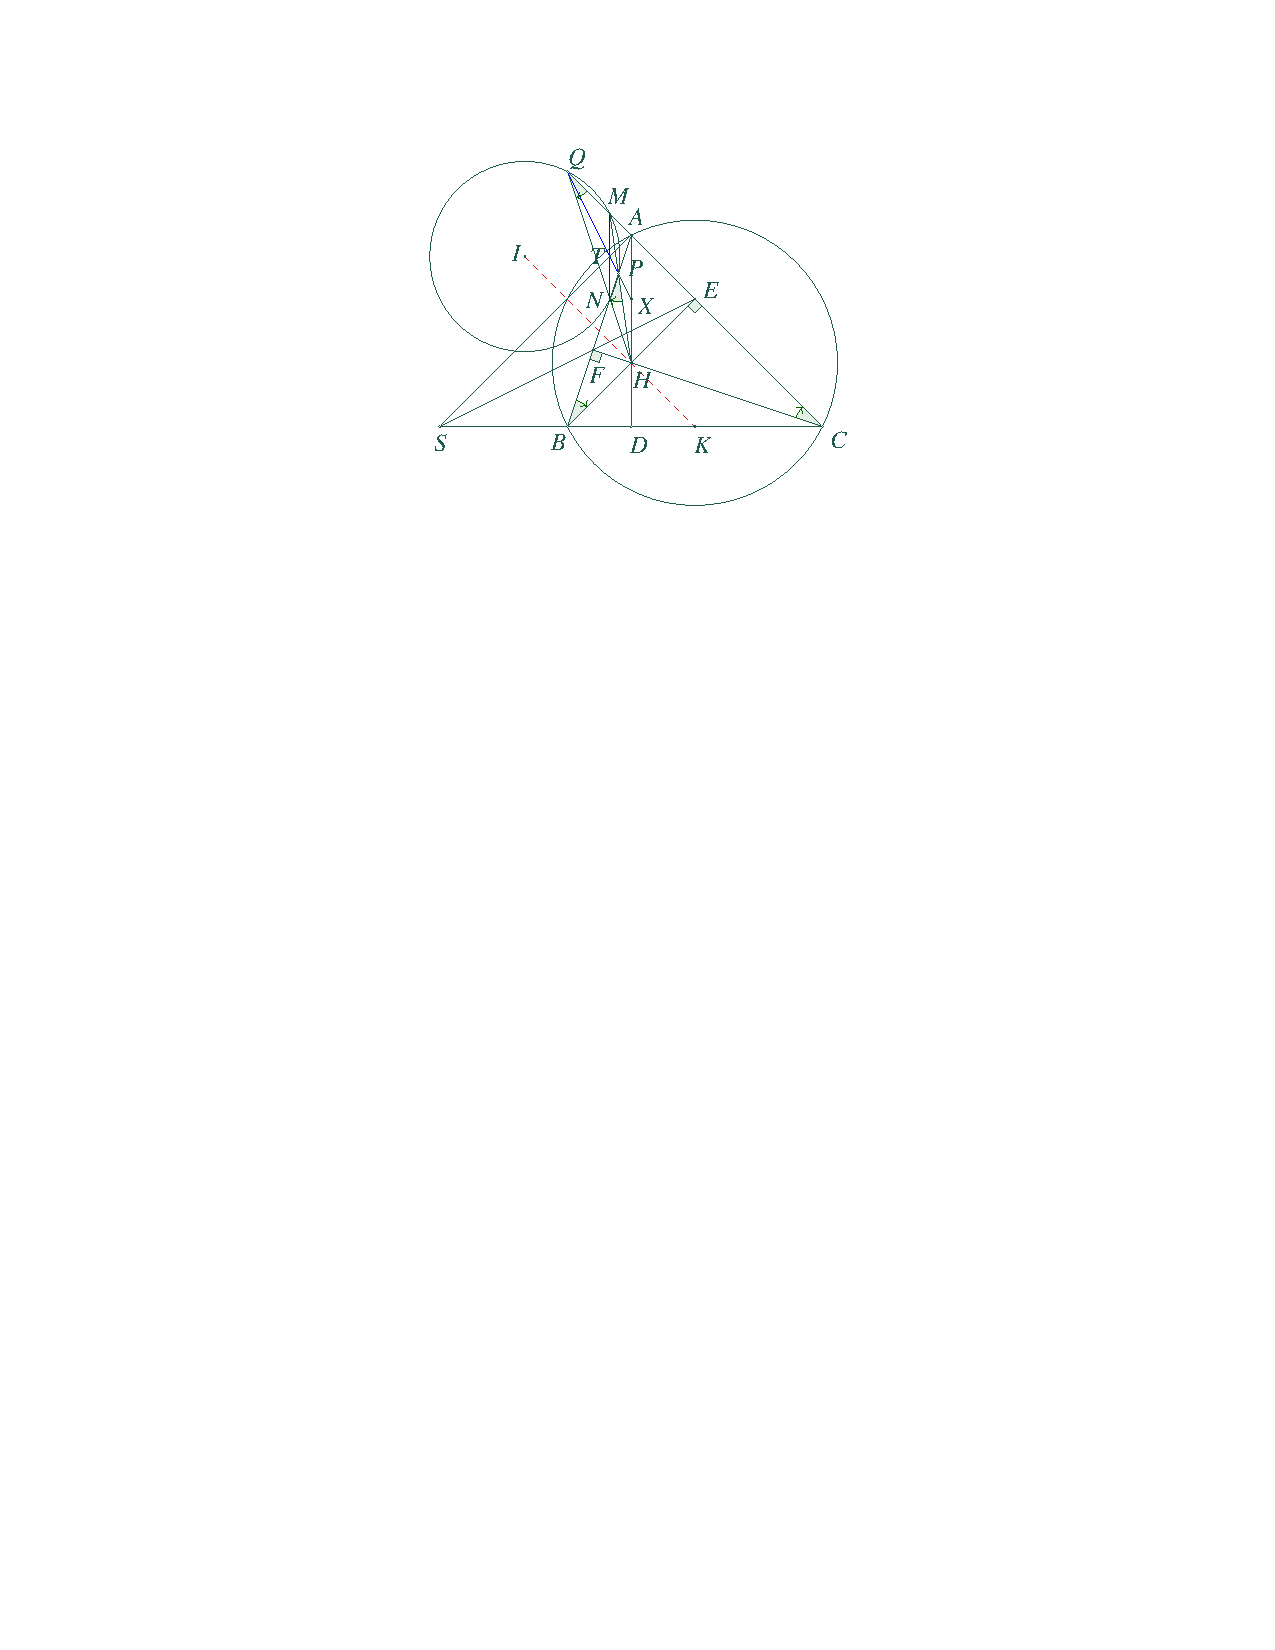
\includegraphics[width=1\linewidth]{P699}
		\vspace*{-15pt}
	\end{figure}
	Do $\angle ABC$  khác $60^\circ$, $90^\circ$   và $120^\circ$, nên bốn điểm $M, N, P, Q$ đôi một phân biệt.
	\vskip 0.05cm
	Do $BE$, $CF$ là các đường cao của tam giác $ABC$, nên bốn điểm $B, C, E, F$ cùng thuộc đường tròn đường kính $BC$. \hfill ($1$)
	\vskip 0.05cm
	Vì thế, với lưu ý tới tính đối xứng của các cặp điểm $(P, B), (Q, C)$, ta có:
	\begin{align*}
			\left( {PM;PN} \right) &\equiv \left( {PH;PB} \right) \equiv \left( {BP;BH} \right) \\
			&\equiv \left( {BF;BE} \right)
			\equiv \left( {CF;CE} \right) \\
			&\equiv \left( {CH;CQ} \right) \equiv \left( {QC;QH} \right)\\
			&\equiv \left( {QM;QN} \right)\left( {\bmod \pi } \right).
	\end{align*}
	Do đó, bốn điểm $M, N, P, Q$ cùng thuộc một đường tròn.
	\vskip 0.05cm
	Gọi $I$ là tâm của đường tròn $(MNPQ)$.
	\vskip 0.05cm
	Gọi $T$ là giao điểm của $MN$ và $PQ$; gọi $S, D$, tương ứng, là giao điểm của $BC$ và $AT, AH$.
	\vskip 0.05cm
	Gọi $X$ là giao điểm của $PQ$ và $AH$. Theo tính chất của tứ giác toàn phần, $(TX, PQ) = -1$. Từ đây, do phép chiếu xuyên tâm bảo toàn tỷ số kép, suy ra $(BC, SD) = -1$.  Vì thế, theo tính chất của tứ giác toàn phần, $S \in EF$.
	\vskip 0.05cm
	Do ($1$) và do $K$ là trung điểm của $BC$ (giả thiết), nên áp dụng định lý Brokard cho tứ giác nội tiếp $BCEF$, ta được $K$ là trực tâm của tam giác $ASH$. Suy ra, $KH \bot AS$. \hfill ($2$)
	\vskip 0.05cm
	Áp dụng định lý Brokard cho tứ giác nội tiếp $MPNQ$, ta được $I$ là trực tâm của tam giác $AHT$. Suy ra, $IH \bot AT$, hay $IH \bot AS$. \hfill ($3$)
	\vskip 0.05cm
	Từ ($2$) và ($3$) suy ra, ba điểm $H$, $K$, $I$ thẳng hàng. Ta có điều phải chứng minh theo yêu cầu đề bài.
	\vskip 0.05cm
	\textbf{\color{thachthuctoanhoc}Bình luận và Nhận xét}
	\vskip 0.05cm
	Tất cả lời giải Tạp chí nhận được từ bạn đọc đều là lời giải đúng.
	\vskip 0.1cm
	\hfill	\textbf{\color{thachthuctoanhoc}Hạ Vũ Anh}
	\vskip 0.1cm
	(Mức $A$) Cho số nguyên dương $n$. Lần lượt ghi các số $n^3,$ $n^3+1,\ldots,$ $n^3+n$ lên $n+1$ tấm thẻ trắng, trên mỗi thẻ ghi đúng một số. Người ta xếp tất cả $n+1$ tấm thẻ đó vào hai chiếc hộp xanh và đỏ, sao cho mỗi hộp có ít nhất một thẻ và  tổng các số được ghi ở các thẻ trong hộp xanh chia hết cho tổng các số được ghi ở các thẻ trong hộp đỏ. Chứng minh rằng, số các tấm thẻ trong hộp xanh chia hết cho số các tấm thẻ trong hộp đỏ.
	\vskip 0.05cm
	\textbf{\color{thachthuctoanhoc}Lời giải} (\textit{dựa trên ý tưởng của bạn Hoàng Nguyễn Gia Bảo, lớp $11$T$1$, trường THPT chuyên Nguyễn Quang Diêu, tỉnh Đồng Tháp})\textbf{\color{thachthuctoanhoc}.}
	\vskip 0.05cm
	Quy ước, gọi tấm thẻ mà trên đó có ghi số $i$ là thẻ $i$.
	\vskip 0.05cm
	$\bullet$ Với $n = 1$, hiển nhiên ta có điều phải chứng minh theo yêu cầu đề bài.
	\vskip 0.05cm
	$\bullet$ Xét $n > 1$.
	\vskip 0.05cm
	Xét một cách xếp $n + 1$ tấm thẻ vào hai hộp xanh, đỏ tùy ý, thỏa mãn điều kiện đề bài.
	\vskip 0.05cm
	Gọi $m$ là số tấm thẻ được xếp vào hộp xanh, và $k$ là số tấm thẻ được xếp vào hộp đỏ; ta có,  $m, k \in \mathbb{N^*}$ và $m + k = n + 1$.
	\vskip 0.05cm
	Ký hiệu  $S_x$ là tổng các số được ghi trên $m$ tấm thẻ trong hộp xanh, và $S_d$ là tổng các số được ghi trên $k$ tấm thẻ trong hộp đỏ; ta có,\linebreak $S_x$, $S_d \in \mathbb{N^*}$  và
	\begin{align*}
		{S_x} + {S_d} &= \left( {n + 1} \right){n^3} + 1 + 2 +  \cdots  + n \\
		&= \left( {n + 1} \right){n^3} + \frac{{n\left( {n + 1} \right)}}{2} \\
		&= \frac{{n\left( {n + 1} \right)}}{2}\left( {2{n^2} + 1} \right). \tag{$1$}
	\end{align*}
	Giả sử $m$ tấm thẻ trong hộp xanh là \linebreak ${n^3} + {x_1}, \ldots ,  {n^3} + {x_m}$; và $k$ tấm thẻ trong hộp đỏ là   ${n^3} + {d_1},\ldots,{n^3} + {d_k}$.
	\vskip 0.05cm
	Đặt $X = {x_1} +  \cdots  + {x_m}$  và  $D = {d_1} +  \cdots  + {d_k}$; ta có:
	\begin{align*}
		&X, D \in \mathbb{N} \text{ và }  X + D = \frac{{n\left( {n + 1} \right)}}{2}, \tag{$2$}\\
		&{S_x} = m \cdot {n^3} + X \text{ và } {S_d} = k \cdot {n^3} + D. \tag{$3$}
	\end{align*}
	Do ${S_x} \,\,\vdots\,\, {S_d}$  (giả thiết), nên tồn tại $q \in \mathbb{N^*}$  sao cho ${S_x} = q{S_d}$. \hfill ($4$)
	\vskip 0.05cm                                                               
	Hơn nữa, từ ${S_x} \,\,\vdots\,\, {S_d}$, dễ dàng suy ra, không thể xảy ra trường hợp trong một trong hai hộp xanh, đỏ, chỉ có duy nhất tấm thẻ $n^3$.  Do đó, từ ($2$) ta có
	\begin{align*}
		X, D \in \mathbb{N^*} \text{ và } X,D < \frac{{n\left( {n + 1} \right)}}{2}. \tag{$5$}
	\end{align*}   
	Vì thế, từ ($3$) suy ra,   ${S_d} > {n^3}.$         \hfill ($6$)
	\vskip 0.05cm
	Từ ($1$), ($4$) và ($6$), ta có:
	\begin{align*}
		\left( {q \!+\! 1} \right){n^3} \!<\! \left( {q \!+\! 1} \right){S_d} \!=\! \frac{{n\left( {n \!+\! 1} \right)}}{2}\left( {2{n^2} \!+\! 1} \right).
	\end{align*}
	Suy ra
	\begin{align*}
		q + 1 &< \frac{{\left( {n + 1} \right)\left( {2{n^2} + 1} \right)}}{{2{n^2}}} \\
		&< n + 2 \,\,(\text{do } n >1);
	\end{align*}
	do đó, $q < n + 1$. Mà  $q \in \mathbb{N^*}$ nên 
	\begin{align*}
		0 < q \le n. \tag{$7$}
	\end{align*}
	Từ ($3$) và ($4$), ta có:
	\begin{align*}
		m \cdot {n^3} + X = qk \cdot {n^3} + qD;
	\end{align*}
	suy ra
	\begin{align*}
		qD - X = \left( {m - qk} \right){n^3}. \tag{$8$}
	\end{align*}
	Do đó, $qD - X$ chia hết cho $n^3$. \hfill ($9$)
	\vskip 0.05cm
	Do ($5$), ($7$), và $n > 1$, nên
	\begin{align*}
		&qD \!-\! X \!<\! qD \!<\! \frac{{{n^2}\left( {n + 1} \right)}}{2} < {n^3}, \tag{$10$}\\
		&qD \!-\! X \!>\! -\! X \!>\! -\! \frac{{n\left( {n \!+\! 1} \right)}}{2} \!>\!  - {n^3}. \tag{$11$}
	\end{align*}
	Từ ($9$), ($10$) và ($11$), suy ra $qD - X = 0$. Vì thế, từ ($8$) ta được $m = qk$; do đó, $m$ chia hết cho $k$. Ta có điều phải chứng minh theo yêu cầu đề bài.
	\vskip 0.05cm
	\textbf{\color{thachthuctoanhoc}Bình luận và Nhận xét}
	\vskip 0.05cm
	$\pmb{1.}$ Lẽ dĩ nhiên, bài đã ra chỉ có ý nghĩa, khi tập các cách xếp thẻ, thỏa mãn điều kiện đề bài, là tập khác rỗng.
	\vskip 0.05cm
	Ở Lời giải trên, ta đã thấy, tập đó khác rỗng, khi $n = 1$.
	\vskip 0.05cm
	Với $n > 1$, dễ dàng kiểm tra được rằng:
	\vskip 0.05cm
	-- Nếu $n$ là số chẵn thì bằng cách xếp thẻ  ${n^3} + \frac{1}{2}n$ vào hộp đỏ, và xếp tất cả $n$ tấm thẻ còn lại vào hộp xanh, ta sẽ có một cách xếp thỏa mãn điều kiện đề bài;
	\vskip 0.05cm
	-- Nếu $n$ là số lẻ thì bằng cách xếp hai thẻ ${n^3} + 1,$ ${n^3} + \left( {n - 1} \right)$   vào hộp đỏ, và xếp tất cả $n - 1$ tấm thẻ còn lại vào hộp xanh, ta sẽ có một cách xếp thỏa mãn điều kiện đề bài.
	\vskip 0.05cm
	Vì vậy, với mọi $n \in \mathbb{N^*}$, tập các cách xếp thẻ, thỏa mãn điều kiện đề bài, là tập khác rỗng.
	\vskip 0.05cm
	$\pmb{2.}$ Trong số các lời giải Tạp chí đã nhận được từ bạn đọc, rất tiếc, có một lời giải sai, do người giải bài đã tính sai tổng các số ghi trên các tấm thẻ trong hộp xanh.
	\vskip 0.1cm
	\hfill\textbf{\color{thachthuctoanhoc}Nguyễn Khắc Minh}
\end{multicols}
\centerline{\textbf{\color{thachthuctoanhoc}DANH SÁCH HỌC SINH CÓ LỜI GIẢI HOÀN CHỈNH}}
\vskip 0.1cm
\textit{Trong các ngoặc đơn ở phần dưới đây, sau tên lớp là mã hiệu của các bài toán mà học sinh có lời giải hoàn chỉnh.}
\begin{multicols}{2}
	\textbf{\color{thachthuctoanhoc}KHỐI THCS}
	\vskip 0.05cm
	$\bullet$  Trường \textbf{\color{thachthuctoanhoc}THPT chuyên Hà Nội -- Amsterdam}, Tp. Hà Nội: \textit{Trần Đăng Hiếu} (lớp $8$A; P$691$), \textit{Hà Mạnh Hùng} (lớp $8$A; P$691$, P$692$, P$693$).
	\vskip 0.05cm
	$\bullet$  Trường \textbf{\color{thachthuctoanhoc}THCS Lê Quý Đôn}, Quận $3$, Tp. Hồ Chí Minh: \textit{Nguyễn Trịnh Phương Minh} (lớp $6/14$; P$691$, P$693$), \textit{Nguyễn Chánh Thiện} (lớp $8/14$; P$691$, P$693$, P$697$).
	\vskip 0.05cm
	$\bullet$  Trường \textbf{\color{thachthuctoanhoc}THCS Nguyễn Trãi}, Thành phố Sơn La, tỉnh Sơn La: \textit{Lương Hữu Bách} (lớp $9$A$1$; P$691$, P$693$, P$697$).
	\vskip 0.05cm
	\textbf{\color{thachthuctoanhoc}KHỐI THPT}
	\vskip 0.05cm
	$\bullet$  Trường \textbf{\color{thachthuctoanhoc}THPT An Lão}, tỉnh Bình Định: \textit{Trần Khánh Duy} (lớp $11$A$1$; P$691$).
	\vskip 0.05cm
	$\bullet$  Trường \textbf{\color{thachthuctoanhoc}THPT chuyên Nguyễn Quang Diêu}, tỉnh Đồng Tháp: \textit{Hoàng Nguyễn Gia Bảo} (lớp $11$T$1$; P$692$, P$700$), \textit{Huỳnh Ngọc Ngân} (lớp $11$T$1$; P$693$), \textit{Đỗ Duy Quang} (lớp $11$T$1$; P$691$, P$693$, P$695$).
	\vskip 0.05cm
	$\bullet$  Trường \textbf{\color{thachthuctoanhoc}THPT chuyên Hà Tĩnh}, tỉnh Hà Tĩnh: \textit{Trần Minh Hoàng} (lớp $10$T$1$; P$697$, P$699$, P$700$).
	\vskip 0.05cm
	$\bullet$  Trường \textbf{\color{thachthuctoanhoc}THPT chuyên Hưng Yên}, tỉnh Hưng Yên: \textit{Trần Hữu Dương} (lớp $11$ Toán $1$; P$691$, P$693$, P$695$), \textit{Nguyễn Gia Khánh} (lớp $11$ Toán $1$; P$699$).
	\vskip 0.05cm
	$\bullet$  Trường \textbf{\color{thachthuctoanhoc}THPT chuyên Lê Hồng Phong}, tỉnh Nam Định: \textit{Ngô Quang Bình} (lớp $11$ Toán $1$; P$695$), \textit{Phùng Việt Cường} (lớp $11$ Toán $2$; P$693$, P$695$, P$696$), \textit{Trần Đình Nam} ($P697$), \textit{Dương Tuấn Phong} (lớp $11$ Toán $2$; P$697$), \textit{Nguyễn Đắc Tú} (lớp $11$ Toán $1$; P$693$).
	\vskip 0.05cm
	$\bullet$  Trường \textbf{\color{thachthuctoanhoc}THPT chuyên Lương Văn Chánh}, tỉnh Phú Yên: \textit{Nguyễn Tấn Nguyên Chương} (lớp $10$ Toán $1$; P$693$, P$699$).
	\vskip 0.05cm
	$\bullet$  Trường \textbf{\color{thachthuctoanhoc}THPT chuyên Lê Thánh Tông}, tỉnh Quảng Nam: \textit{Ngô Gia Tưởng} (lớp $10/1$; P$697$).
	\vskip 0.05cm
	$\bullet$  Trường \textbf{\color{thachthuctoanhoc}THPT chuyên Quốc học Huế}, tỉnh Thừa Thiên -- Huế: \textit{Trần Thị Thanh Thư} (lớp $12$T$1$; P$693$).
	\vskip 0.05cm
	$\bullet$  Trường \textbf{\color{thachthuctoanhoc}THPT chuyên Tiền Giang}, tỉnh Tiền Giang: \textit{Huỳnh Nguyễn Khánh Duy} (lớp $10$ Toán; P$698$, P$699$, P$700$), \textit{Trần Phúc Thịnh} (lớp $10$ Toán; P$691$).
	\vskip 0.05cm
	$\bullet$  Trường \textbf{\color{thachthuctoanhoc}THPT chuyên Tự nhiên}, ĐH KHTN -- ĐHQG Hà Nội: \textit{Vương Khánh Toàn} (lớp $10$A$1$ Toán; P$697$, P$700$).
	\vskip 0.05cm
	$\bullet$  Trường \textbf{\color{thachthuctoanhoc}THPT chuyên Sư phạm}, ĐH Sư phạm Hà Nội: \textit{Hồ Trần Khánh Linh} (lớp $12$ Toán $2$; P$698$, P$699$).
\end{multicols}
\vspace*{-10pt}
{\color{thachthuctoanhoc}\rule{1\linewidth}{0.1pt}}
\vskip 0.4cm
\centerline{\LARGE{\color{thachthuctoanhoc}\textbf{LỜI GIẢI, ĐÁP ÁN}}}
\vskip 0.2cm
\begin{multicols}{2}
	\textbf{\color{thachthuctoanhoc}Hai băng cướp bị tóm gọn}
	\vskip 0.1cm
	Đối với mỗi tên thuộc băng Mèo rừng ta sẽ đánh dấu bằng màu đỏ tên cướp thuộc băng Báo đen nào to béo nhất ngồi cạnh hắn ta (nếu hai tên Báo đen nặng như nhau ngồi cạnh, ta sẽ chọn lấy đúng một tên bất kỳ; hoặc nếu chỉ có một tên Báo đen ngồi cạnh thì ta sẽ chọn đúng tên đó). Như vậy mỗi tên cướp ở băng Báo đen được đánh dấu sẽ ngồi cạnh một tên thuộc băng Mèo rừng gầy còm hơn hắn ta.
	\vskip 0.1cm
	Giả sử không phải tất cả các tên thuộc băng Báo đen được đánh dấu đỏ. Khi đó số các tên thuộc băng Báo đen được đánh dấu sẽ nhỏ hơn hoặc bằng $9$. Vì mỗi tên thuộc băng Báo đen chỉ có thể ngồi cạnh không quá $2$ tên thuộc băng Mèo rừng, suy ra bên cạnh các tên cướp được đánh dấu đỏ thuộc băng Báo đen có không quá $18$ tên thuộc băng Mèo rừng, số lượng này ít hơn tổng số các tên cướp thuộc băng Mèo rừng là $19$ tên. Ta nhận được mâu thuẫn, do tất cả các tên cướp thuộc
	băng Mèo rừng đều phải ngổi cạnh một tên thuộc băng Báo đen được đánh dấu đỏ.
	\vskip 0.1cm
	Như vậy, mỗi tên thuộc băng Báo đen phải có một tên thuộc băng Mèo rừng gầy còm hơn ngồi cạnh.
	\vskip 0.1cm
	\textbf{\color{thachthuctoanhoc}Đố vui}
	\vskip 0.1cm
	Bản nhạc trên hành tinh Vui vẻ có nhiều nhất là $16$ nốt nhạc, cho bởi  
	\begin{align*}
		AABABAABABAABAAB
	\end{align*}
	hoặc dãy ngược lại. Còn bạn thì sao?
\end{multicols}
